\section{Implementation}
\label{sec:implementation}

\IEEEPARstart{I}{n} this chapter, we present the design and implementation of the different preconditioners and solvers that we developed, and we provide details about how we integrated them and other third-party GPU libraries into OPM Flow. 

\subsection{OPM Flow}
OPM Flow is composed of two main parts: the assembly and the linear solve. The linear solve is performed by the dune-istl\cite{dune-istl} iterative solver template library. 
OPM uses an ILU0 preconditioned BiCGStab solver as the default configuration. 
When the wells are added to the matrix, it performs the standard bicgstab algorithm.
When the wells are separate, the linear operation (spmv) in the bicgstab is replaced by a combination of an spmv and an operation to apply the wells.
This operation is defined in opm-simulators.
Dune-istl is able to handle blocks of all sizes.

During initialization, the bridge verifies that the implementation specified on the command line is available and creates the chosen backend solver.

Right before dune-istl is called, our bridge tries to solve the linear system.
At this point, the linear system is stored in the dune-istl BCRS matrix and block vector format.
The block vector has a contiguous array internally, storing all the values.
This is easily copied to the GPU.
The matrix has three components: nonzero values, row pointers, and column indices.
The nonzeroes are blocked; Figure \ref{fig:amgcl_layout} shows how they are stored in memory.
Due to the construction of the matrix in opm-simulators, the nonzeroes are stored contiguously.
These are also easily copied to the GPU, but a check must be made to ensure they are indeed contiguous.
The row pointers and column indices are not readily available.
To get them, the matrix is iterated through, and the sparsity pattern is written to two contiguous arrays.

The linear system is solved via a preconditioned bicgstab solver, capable of handling 3x3 blocks.
If the backend solver is unsuccessful, the call to dune-istl is still made; see subsection \ref{sec:fallback}.

\subsection{Bicgstab solver}
The bicgstab solver needs some basic functions like spmv, axpy, norm, and dot.
The spmv implementation is described in \ref{lab:spmv}.

For the norm and dot, the GPU kernel only returns partial sums, which are added to the CPU.
Each work item calculates the result of one row, and the workgroup reduces this to one value in local memory.
The function $work\_group\_reduce\_add()$ from Opencl 2.0 was not available, since Opencl 1.2 needs to be supported for NVIDIA GPUs.

The default stopping condition in Dune is a relative reduction in error of $0.01$, with a maximum number of linear iterations of $200$.
Our implementation allows us to pass the same stopping criteria with the same default values.

\subsection{Sparse Matrix-Vector multiplication}
\label{lab:spmv}
A sparse matrix-vector multiplication (spmv) multiplies a sparse matrix A with a dense vector x, resulting in a dense vector y.
Each row i of A can be seen as a sparse vector, and then the inner product between row i and vector x can be calculated to form entry $y_i$.
Every element of y can be calculated in parallel since they do not have dependencies.
For OPM, the elements of A are actually small, dense blocks of size NxN, and elements of x and y are small, dense vectors of size N.
The sparse inner product becomes more complex: the two scalar elements $a_{ij}$ and $x_j$ are now a dense matrix and a dense vector.
To multiply, a standard dense matrix-vector multiplication is performed.

To implement this on the GPU, Algorithm 1 from \cite{blocked_spmv} is used:
Each warp or workgroup is assigned to one or more blockrows.
The warp then iterates through them until all are processed.
For a particular block row, the warp covers 32/bs$^2$ blocks at a time, where bs is the block size.
For a block size of 3, the warp covers 3 blocks with 27 threads or workitems, and 5 are left idle.
The thread's position inside a block does not change, it only moves to the same position in another block.
Each thread has its own running sum, row (r), and column (c) inside the block.
It multiplies its element from the block with the corresponding element of x, adding it to the running sum.
It then moves to the next block, which is actually 32/bs$^2$ blocks over.
Once the warp has iterated through all blocks in the row, threads that have the same r in the block reduce their running sums into one combined sum, which is written to the output vector.
The paper assumes the values inside the block are stored column-major, but the blocks in OPM are generated by Dune\cite{dune}, which are row-major. This does not change the way the algorithm works; during reading the element of A, the row and column of a thread are simply swapped.

\subsection{ILU0}
ILU0 has two phases: decomposition/creation and application.
During the decomposition, Incomplete LU factorization without fill-in is performed.
To apply the preconditioner, two triangular solves have to be performed with the resulting L and U factors.
Since the sparsity pattern does not change throughout the simulation, the information derived from it can be reused.
The sparsity pattern dictates the amount of parallelism that can be extracted from it.
There are two implemented options to extract parallelism: level scheduling (LS) and graph coloring (GS).
For debugging purposes, performing the ILU sequentially is also an option.
Level scheduling respects indirect dependencies, whereas graph coloring is more aggressive and does not.
If row C depends on row B, and row B depends on row A, then row C indirectly depends on row A.
With LS, row C will be processed after row A is done.
With GC, these two rows will be assigned the same color and processed simultaneously.
All rows that are processed in parallel are in the same level or color.

After extracting the parallelism, a reordered copy of the matrix is made.
In here, the rows of the matrix are reordered, such that all rows in the same color are in contiguous memory.
The column indices are reordered accordingly.
The $b$ is also reordered.
To perform the GPU kernels, the technique in \cite{blocked_spmv} was used.
This paper describes an spmv operation, but this can also be used for the ILU0 decomposition and application.
During the execution of the decomposition and application, each color is processed by a new kernel launch.

\subsection{Block-Jacobi-ILU0}
\label{lab:blockjacobi}
ILU0 is a powerful preconditioner and an important part of the linear solver.
A drawback is that it is fairly slow, a large amount of time is spent in the decomposition and application phases, especially on GPU.
Other parts of the linear solver can be parallelized relatively easily, but ILU0 is an inherently sequential algorithm because the rows depend on each other.
This can be solved by using LS or GC, but the ILU part of the solver can still be the bottleneck.

To further increase parallelism, dependencies can be removed from the decomposition matrix.
The original matrix should still be used for the rest of the solver.
Removing blocks from the matrix for the preconditioner should be done in a smart way to reduce the quality of the preconditioner as little as possible while still improving parallelism.
When using N MPI processes to run Flow, the grid can be partitioned into N partitions.
Each partition will be assembled and solved in parallel, with some extra computation and synchronization for the boundary between the partitions.
The partitions are created according to the transmissibilities between cells, these indicate how tightly the cells are coupled.
More information can be found in \cite{Thune_2021}.

The GPU implementation of the Block-Jacobi-ILU0 preconditioner uses the same partitioning algorithm, but the number of partitions is set by the user.
Since every row in the matrix corresponds to an active cell in the grid, it is easy to remove blocks that represent a connection between two cells belonging to different partitions.
These functions are inspired by the work in \cite{andreas}.
This new matrix is then used for the ILU preconditioner.
The sparsity pattern is analyzed, and since it contains fewer blocks, it can extract more parallelism.
The convergence of the ILU preconditioner is not affected too much if the number of partitions is low enough and if the partitioning is done in a smart way (using the transmissibilities).

The Jacobi matrix has the same number of rows and columns, but less nonzero blocks. To allow the matrix nonzeroes to be copied by a single GPU copy, they must be stored in contiguous memory. The Dune::BCRSMatrix allocates contiguous memory when the maximum number of nonzeroes is passed to the constructor. The number of nonzeroes in the full matrix serves as this upper bound.
For every linear solve, blocks must be copied from the full matrix to the Jacobi matrix.
This can be done by iterating the two matrices simultaneously and copying a single block when a match is found in the sparsity pattern.
Alternatively, since the nonzeroes of both matrices are stored in contiguous memory, the indices of the blocks that need to be copied can be stored in a big vector $indices$. Each nonzero block gets its own entry in that vector. Copying then occurs in a single loop:
\begin{algorithm}
\caption{Copy indexes}
\begin{algorithmic}
\STATE for i in indices: 
\STATE \hspace{0.5cm}jacobi\_matrix\_nnzs[i] = full\_matrix\_nnzs[indices[I]]
\end{algorithmic}
\end{algorithm}

\subsection{Well Contributions}
The default CPU implementation does not actually perform a standard bicgstab solver.
After the spmv operation, a separate function is performed to incorporate the contributions of all active wells.
A runtime parameter exists to put these contributions inside matrix A itself, allowing a standard bicgstab solver to be used.
This will increase the complexity of the matrix and might deteriorate converge performance.
This function is described in Algorithm \ref{alg:wells_coupled}.
When the wellcontributions are kept separate, they are added like in Algorithm \ref{alg:wells_separate}.
The spmv from the bicgstab solver is put in a comment.

\begin{algorithm}
\caption{Adding the wellcontributions to matrix A}
\begin{algorithmic}
\STATE for well in wells: \\
\STATE \hspace{0.5cm}A = A - well.C$^T$ * well.D$^{-1}$ * well.B \\
\end{algorithmic}
\label{alg:wells_coupled}
\end{algorithm}

\begin{algorithm}[H]
\caption{Adding the wellcontributions separately}
\begin{algorithmic}
\STATE y = A * x 
\STATE for well in wells: \\
\STATE \hspace{0.5cm}t1 = well.B * x \\
\STATE \hspace{0.5cm}t2 = well.D$^{-1}$ * t1 \\
\STATE \hspace{0.5cm}y = y - well.C$^{T}$ * t2 \\
\end{algorithmic}
\label{alg:wells_separate}
\end{algorithm}

For standard wells:
\begin{itemize}
\item D is a single block
\item B and C have 1 row, with a nonzero block at (0,j) if this well has a perforation at cell j
\end{itemize}

For multisegment wells:
\begin{itemize}
\item nseg is the number of segments of that well
\item D is a (nseg x nseg) dense block matrix
\item B and C are (nseg x ncells) sparse block matrices, they have a block at (i, j) if this well has a perforation at cell j connected to segment i. The columns of B/C have no more than one nonzero block.
\end{itemize}

To allow separate wellcontributions for standard wells on the GPU, manual kernels have been written to apply them.
The variables B, C, and D can be interpreted as sparse vectors since they have only one row.
There are three contiguous arrays, which store the B, C, and D of all the wells.
For D, the inverse D$^{-1}$ is stored instead, since multiplying with the inverse is easier.
These three arrays are copied to the GPU.
The CUDA and OpenCL kernels for standard wells apply to all wells in parallel.
For every well, one workgroup is launched.

The multisegment wells are more complex; they have more, irregular-sized data, and are applied using UMFPack\cite{umfpack} on the CPU.
Their application is not implemented on the GPU; instead, the x and y vectors are copied to the CPU, where they are applied with UMFPack.
The resulting y vector is then copied back to the GPU.

\subsection{Amgcl}
Amgcl\cite{amgcl1,amgcl2} is a header-only C++ library for solving (blocked) sparse linear systems.
It features different preconditioners and iterative solvers.
Different backends like OpenMP, CUDA, or OpenCL can be used.
All these different configurations can be chosen at runtime.
It can also connect to VexCL\cite{vexcl}, ViennaCL, Eigen\cite{eigen} and Blaze\cite{blaze}.

The memory layout for blocked matrices in amgcl is different from OPM, as described in Figure \ref{fig:amgcl_layout}.
This means that for every linear solve, the matrix must be transformed to be used by amgcl.

\begin{figure}
\centering
\begin{tabular}{cccccc|cccccc}
0 & 1 & 2 & 9 & 10 & 11     &   0 & 1 & 2 & 3 & 4 & 5 \\
3 & 4 & 5 & 12 & 13 & 14     &  6 & 7 & 8 & 9 & 10 & 11 \\
6 & 7 & 8 & 15 & 16 & 17     &  12 & 13 & 14 & 15 & 16 & 17 \\
\end{tabular}
\caption{Memory layout of blocks in OPM (left) and amgcl (right).}
\label{fig:amgcl_layout}
\end{figure}

To use amgcl, the wellcontributions must be included in the matrix.

\subsection{Rocalution}
Rocalution\cite{rocalution} is a sparse linear algebra library.
It focuses on utilizing fine-grained parallelism and is built on top of AMD's ROCm\cite{rocm} ecosystem.
Numerous iterative solvers, preconditioners, and sparse matrix formats are supported.
It is designed to be able to run on both NVIDIA and AMD GPUs.

The memory format for blocked matrices is row-major, like Dune's BCRSMatrix.
However, the nonzero values inside the blocks must be column-major.
This means that for every linear solve, every matrix block must be transposed before sending it to rocalution.

It does have a BlockJacobi preconditioner, similar to the one described in Subsection \ref{lab:blockjacobi}.
However, it requires the use of GlobalMatrix, a distributed matrix that does not have an easy way to handle blocked matrices.
It also doesn't have a way to determine the blocks manually.
Using the transmissibilities to partition helps to reduce the loss in convergence power.

To use rocalution, the wellcontributions must be included in the matrix.
It might be possible to extend the Operator class, and both apply spmv and add the wellcontributions in its apply() function, but this might break the bicgstab solver and has not been tried yet.

\subsection{cuSPARSE}
cuSPARSE\cite{cusparse} is a library with basic linear algebra functions used for handling sparse matrices.
It is created by NVIDIA and is implemented on top of the CUDA runtime.
Since the bicgstab solver also uses some dense vector functions, cuBLAS\cite{cublas} is used in combination with cuSPARSE to create cusparseSolver.

A CUDA kernel is written to apply the standardwell contributions for cusparseSolver, so that including them in the matrix is not required.
Multisegment wells are still applied on CPU.

\subsection{Rocsparse}
Rocsparse\cite{rocsparse} is the sparse linear algebra implementation of the ROCm framework.
It has the same interface as cusparse.
Using the building blocks provided in the library and the dense vector functions from rocblas, a simple ILU0-BiCGStab solver can be constructed.
The advantage of using rocsparse over rocalution is that the Block-Jacobi-ILU0 preconditioner can be used.
It should also be easier to allow for separate wellcontributions applications.

\subsection{Fallback}
\label{sec:fallback}
If the chosen BdaSolver fails to converge within the specified limits (default 200 linear iterations), the simulation will fall back to the CPU Dune implementation.
The ILU0 decomposition is performed, and the solver is started.

The ILU0 decomposition from the chosen BdaSolver might be able to be reused instead since it has already been performed.
Only the copying added time and could be faster than the CPU ILU0 decomposition.
Since fallbacks are relatively rare, this is not implemented.

\begin{figure*}[!t]
\centering
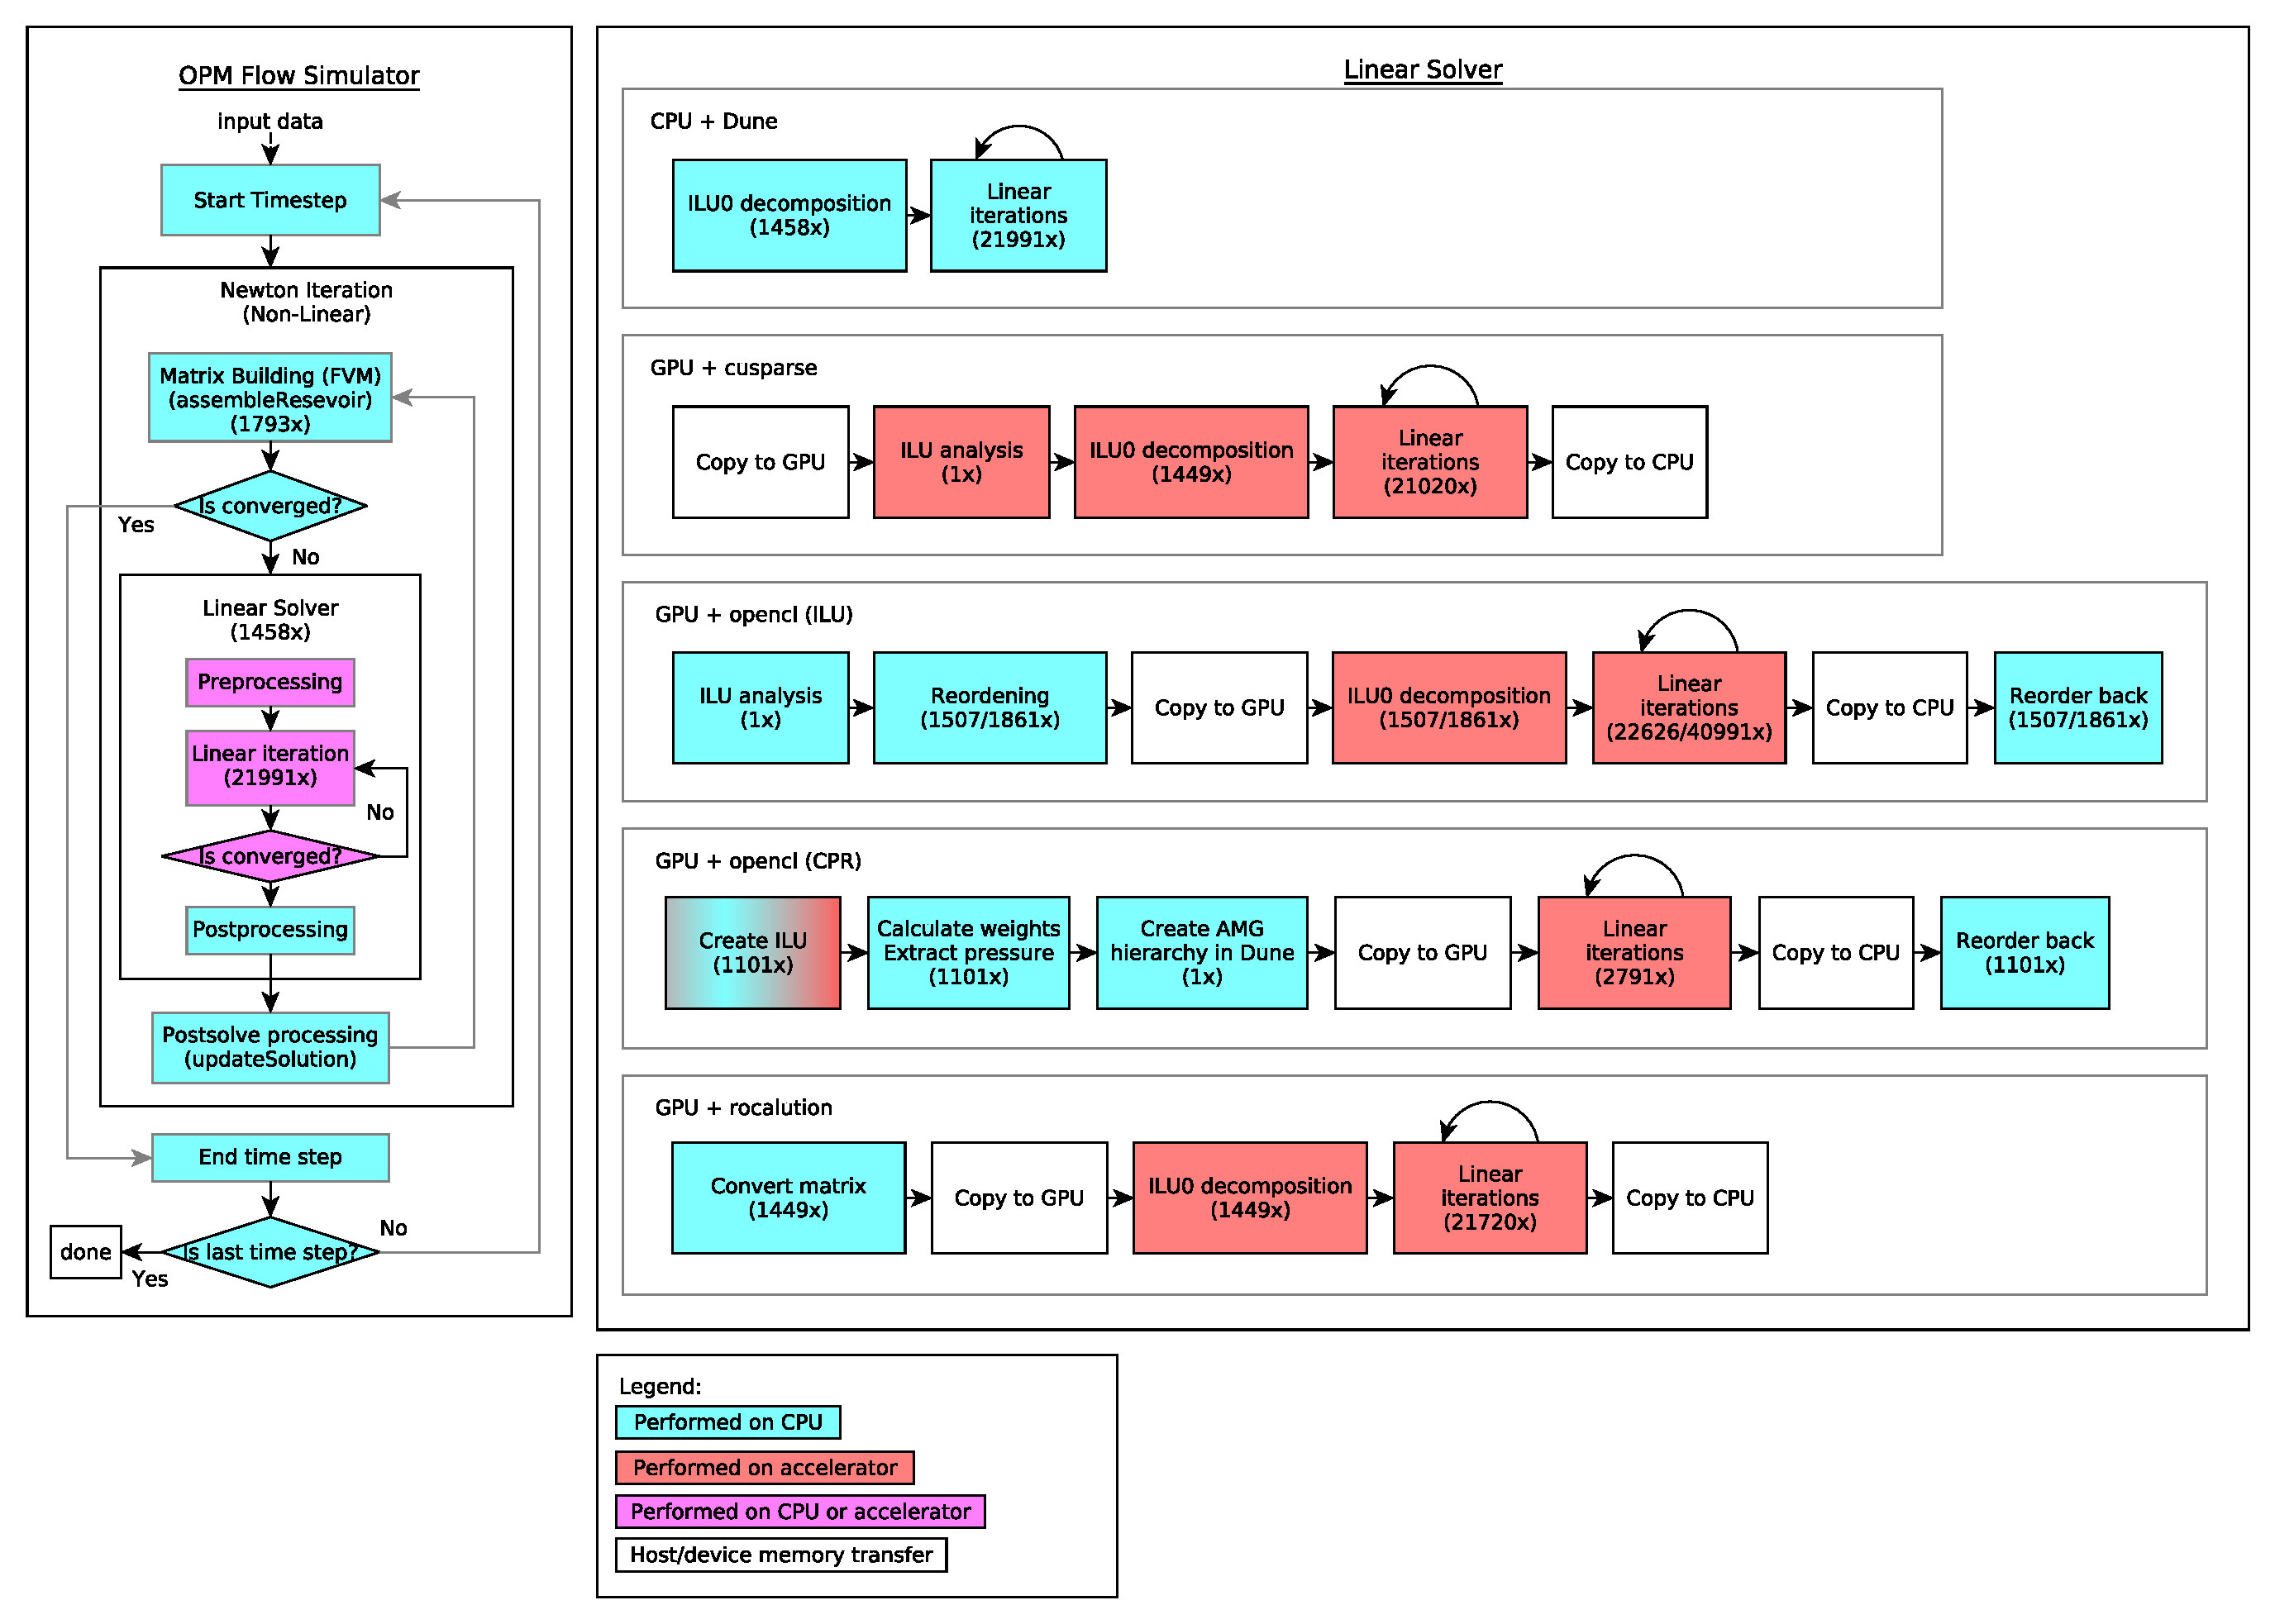
\includegraphics[width=0.65\textwidth]{figures/Flow_simulator_overview.pdf}
\label{fig:flow_chart2}
\caption{The flowchart of different implementations.}
\end{figure*}

